\chapter{Epipolar Attention in NeRF}
\label{chapter:epinerf}


\chapterwithfigures{\nameref*{chapter:epinerf}}
\chapterwithtables{\nameref*{chapter:epinerf}}

\ifthenelse{\boolean{skipEpiNeRF}}{\endinput}{}


\section{Introduction}


Few-shot NVS presents a challenging task in computer vision, wherein the objective is to generate an image from an unobserved viewpoint using only a limited number of source images and their corresponding camera pose information. The present work addresses an even more intricate scenario, which exclusively relies on a unique source image. The problem is inherently ill-posed as a single source image may not provide enough visual clues to generate a novel viewpoint. Handling unforeseen elements as well as occlusions becomes particularly challenging in this scenario. To effectively tackle these challenges, leveraging 3D priors \citep{saito2019pifu,johari2022geonerf} is fundamental since it enables deep architectures to acquire a primary understanding of the underlying 3D scene structure. 

Recent advances in neural rendering \citep{tewari2022advances} significantly drive latest works in the few shot NVS issue. While original neural radiance field (NeRF) \citep{mildenhall2020nerf} allows to represent a scene through a learned overfitted 5D function, it does not have any generalization abilities. Latest contributions \citep{yu2021pixelnerf,li2022symmnerf,lin2023vision} designed low-resolution 2D feature \textbf{F} conditioning to tackle such a limitation, mostly by leveraging on an image encoder. Produced feature volume is sampled at training and testing time through pixel-aligned bilinear interpolation to \textit{locally} condition the radiance field. However, the deep feature is aligned with the source view: occlusions and unobserved parts therefore lead to misaligned and coarsely-local feature sampling on \textbf{F}, producing non-optimal conditioning. 

\begin{figure}[htp!]
    \center
  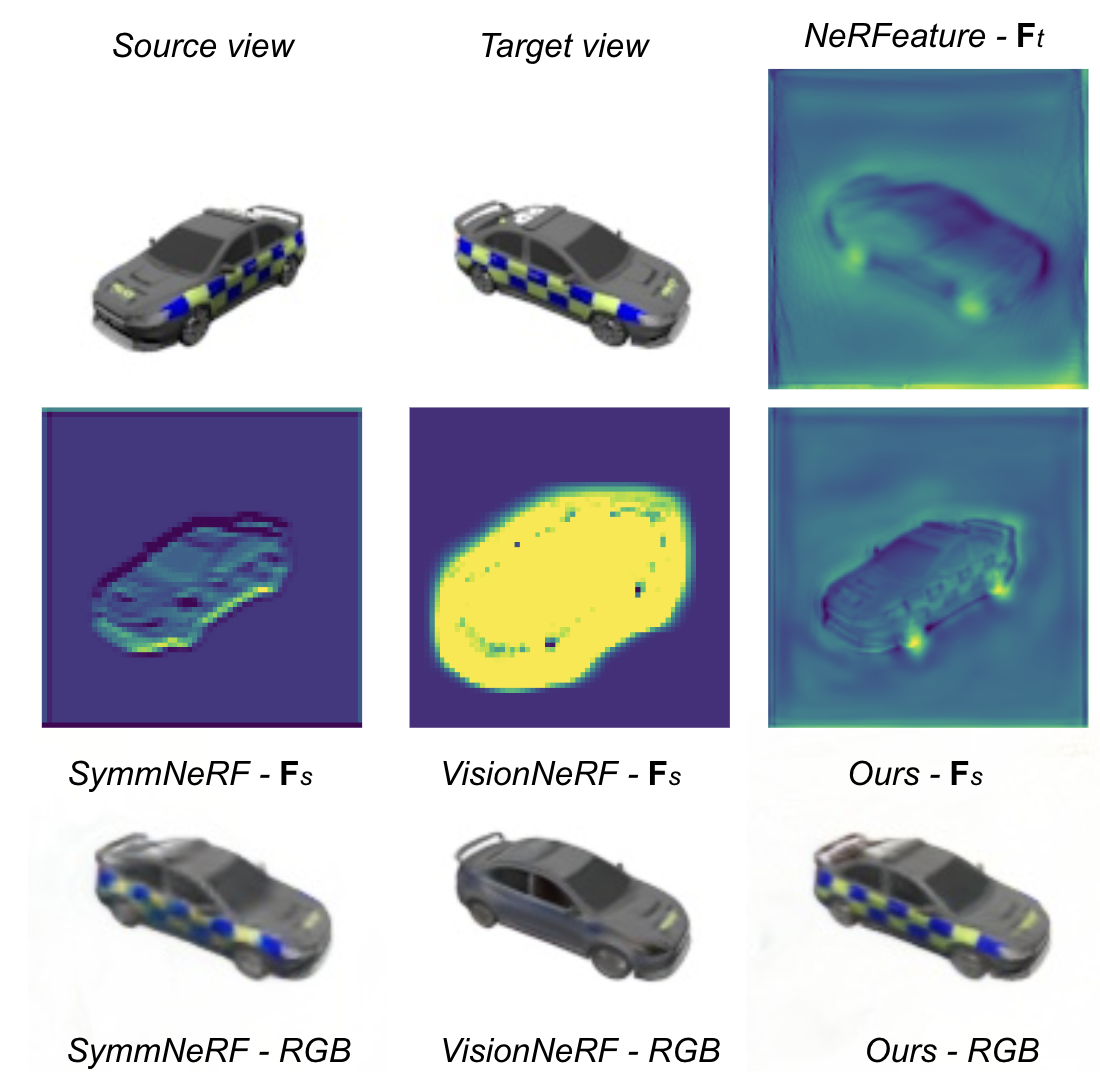
\includegraphics[width=.65\textwidth]{images/epinerf/abstract_figure.png}
  \caption{Comparison with state-of-the-art methods, both in RGB space as well as on feature space. Existing methods rely only on source-aligned features. In contrast, the proposed method uses both a source and a target-aligned features to predict the image associated to the target view, leading to a better quality rendering. In this example, VisionNeRF \citep{lin2023vision} correctly synthesised the rear wing, but fails to render the yellow and blue checkerboard painted on both car' sides. If SymmNeRF \citep{li2022symmnerf} manages to reproduce such a pattern, it lacks details on the rear wing too.}
  \label{fig:res_car_intro}
\end{figure}

Our work therefore try to address such limitations by producing target-aligned features from a feature radiance field, called NeRFeature. Associated training is supported through a light feature distillation procedure, by leveraging on a CNN encoder-decoder as teacher network. Target oriented feature (from the NeRFeature student radiance field) is then involved (with its source-aligned counterpart) in an epipolar-based attention mechanism: it shrinks the weights sampling distribution around regions where source and target features match, allowing better sampling during neural rendering. Corresponding results, both in RGB and feature space can is illustrated on Figure \ref{fig:res_car_intro}. We conducted extensive ex\--periments and ablations studies to motivate our claims, whereas our architecture outperforms most of current state-of-the art methods on the ShapeNet dataset \citep{chang2015shapenet}. Our contributions are threefold and can be summarised through: 
\begin{enumerate}
   \item A learned feature radiance field, called NeRFeature. Given a source-aligned feature and a camera transformation, NeRFeature aims to infer the correspond\--ing target-aligned deep feature trough a light feature distillation procedure, that do not involve any heavy foundation models (section \ref{subsec:nerfeature}). 
    \item A simple yet effective epipolar-based attention mechanism that relies on source and target aligned features and which adjust the weights sampling distribution during volume rendering (section \ref{subsec:epipolar_att}). 
    \item A novel generalizable NeRF architecture for single-image NVS, EpiNeRF, \textit{locally} conditioned on its input with a CNN as well as \textit{globally} conditioned on its weights through a Hypernetwork (section \ref{subsec:epinerf}).  
\end{enumerate}

\section{Related work}

\noindent\textbf{Single-image novel view synthesis.} Novel view synthesis aims to render an image of a scene from a an unobserved viewpoint, given a set of posed images, i.e. images and the associated camera poses (3D position and orientation). NVS has been widely studied over the last few decades from both graphics and computer vision perspectives. Early pioneer works \citep{chen93view,levoy96light,fitzgibbon2005image} mostly relied on graphics and multi-view geometry concepts, such as light field, warping or blending operations to synthesise novel view. However, synthesising a viewpoint from a different location based on a single image is an ill-posed task. Occluded parts cannot be easily recovered in this scenario, as the 3D scene cannot be triangulated. The recent breakthrough of deep networks has opened the door for learning-based methods. While fully convolutional-based networks first appeared in the devoted literature \citep{zhou2016view,sun2018multi,kim2020novel,hou2021novel,guo2022fast,landreau2022epipolarnvs}, the emergence of neural radiance fields \citep{mildenhall2020nerf} and neural rendering \citep{tewari2022advances} highly influenced the way single-view novel view synthesis architectures \citep{yu2021pixelnerf,li2022symmnerf,lin2023vision} are built. Introducing explicit 3D concepts (regarding camera pose, implicit or neural 3D reasoning etc) within architectures significantly help deep neural networks to better address such 3D vision task relying on implicit representations. Latest research directions in single-image NVS pushes toward extremely large deep networks, such as image-conditioned diffusion models\citep{chen2023single,xiong2023light,chan2023genvs,yu2023long}. Note that, recent advances in large 3D reconstruction \citep{hong2023lrm} use even bigger models, that are able to explicitly grasp the whole 3D structure of an object from a single view \citep{liu2023zero,shi2023zero123++,liu2024one,liu2023one2345++,zou2023triplane}. However, these diffusion-based architectures remain complex to train and have poor speed inference performances.  

\noindent\textbf{3D Geometry prior in single-image NVS.} Few works attempted to integrate geometrical priors within their single-image NVS architecture. Whereas Epipolar\--NVS \citep{landreau2022epipolarnvs} directly incorporates the geometrical camera transformation through a finite set of epipolar lines, SymmNeRF \citep{li2022symmnerf} integrates a symmetrical constraint with a simple yet effective assumption in the canonical coordinates system. 
\newline

\noindent\textbf{Generalizable NeRF conditioning.} Introduced in Mildenhall's \etal \citep{mildenhall2020nerf} work, a neural radiance field $\psi$ aims to implicitly represent the inherent geometry and appearance of a scene. In its original formulation, a set of posed images $\{I,\pi = K[R|t]\}$ is sufficient to learn such a radiance field. Given a 3D point in world space $\mathbf{x} \in \mathbb{R}^{3}$ along a ray and its viewing direction $\mathbf{d} \in \mathbb{R}^{3}$, a vanilla RGB radiance field is entirely defined through its density $\sigma_{\psi}(\mathbf{x})\in \mathbb{R}_{+}$  and an RGB colour $c_{\psi}(\mathbf{x},\mathbf{d}) \in \mathbb{R}^{3}$. 
A differentiable volume rendering operation \citep{max1995optical} is performed to render the final composite RGB color $\hat{c}$ along the ray. 

However, this formulation prevents $\psi$ to generalise across multiple scenes. While plethora works nowadays rely on deep feature volume to condition their neural architecture \citep{saito2019pifu,wang2021ibrnet,chen2023matchnerf}, PixelNeRF \citep{yu2021pixelnerf} has paved the way to such limitation in single-image NVS. It locally conditions its radiance field using pixel-wise source aligned features, obtained from a CNN encoder-decoder. 

Such a $d_{\text{feat}}$-dimensional pixel-aligned feature is obtained through the perspective projection of a 3D point onto the  source-aligned feature volume.

\begin{equation}
    c_{\psi} \colon \mathbb{R}^{3}\times\mathbb{R}^{3}\times\mathbb{R}^{d_{\text{feat}}}  \longrightarrow \mathbb{R}^{3}  \\
    \textbf{x},\textbf{d}, f  \longmapsto  c_{\psi}(\textbf{x},\textbf{d}, f)
\end{equation}


Such a \textit{local} -input based- conditioning is now commonly adopted in devoted literature \citep{jang2021codenerf,li2022symmnerf,lin2023vision}, even through VisionNeRF \citep{lin2023vision} also claims a \textit{global} input conditioning of its radiance field through a vision transformer (ViT) \citep{dosovitskiy2020vit} they embedded in their architecture. \newline

\noindent\textbf{Feature distillation in NeRF.} A radiance field can be extended to output additional features of interest, and thus go beyond RGB space, as soon as a supervisory signal exists to train such an architecture. Several approaches can thus be derived from the original neural radiance fields seminal work, including BRDF-based methods \citep{boss2021nerd,verbin2022ref}, deep latent feature-based methods \citep{kobayashi2022decomposing,ye2023featurenerf,chan2023genvs}, or even methods that are parametrized to handle dynamic scenes \citep{pumarola2021d,yan2023nerf}. From a feature distillation perspective, research from \citep{hinton2015distilling} paved the way, mostly to tackle both knowledge transfer and model compression issues. Few works already attempted to distill feature from a 2D model (such as a CNN or a ViT) into 3D through the use of neural radiance fields \citep{kobayashi2022decomposing, tschernezki2022neural}. \citep{ye2023featurenerf} is the closest work, regarding our first contribution consisting in learning feature radiance field in the spirit of a teacher-student framework. However, the authors in \citep{ye2023featurenerf} distilled learned feature from a 2D foundation model \citep{oquab2023dinov2} while we propose a lighter feature distillation procedure. 

\section{Method}

We present an overview of our architecture on Figure \ref{fig:overview}. Following subsections are devoted to the different sub-modules EpiNeRF has and how they have been built.
\begin{figure*}[htb!]
    \center
  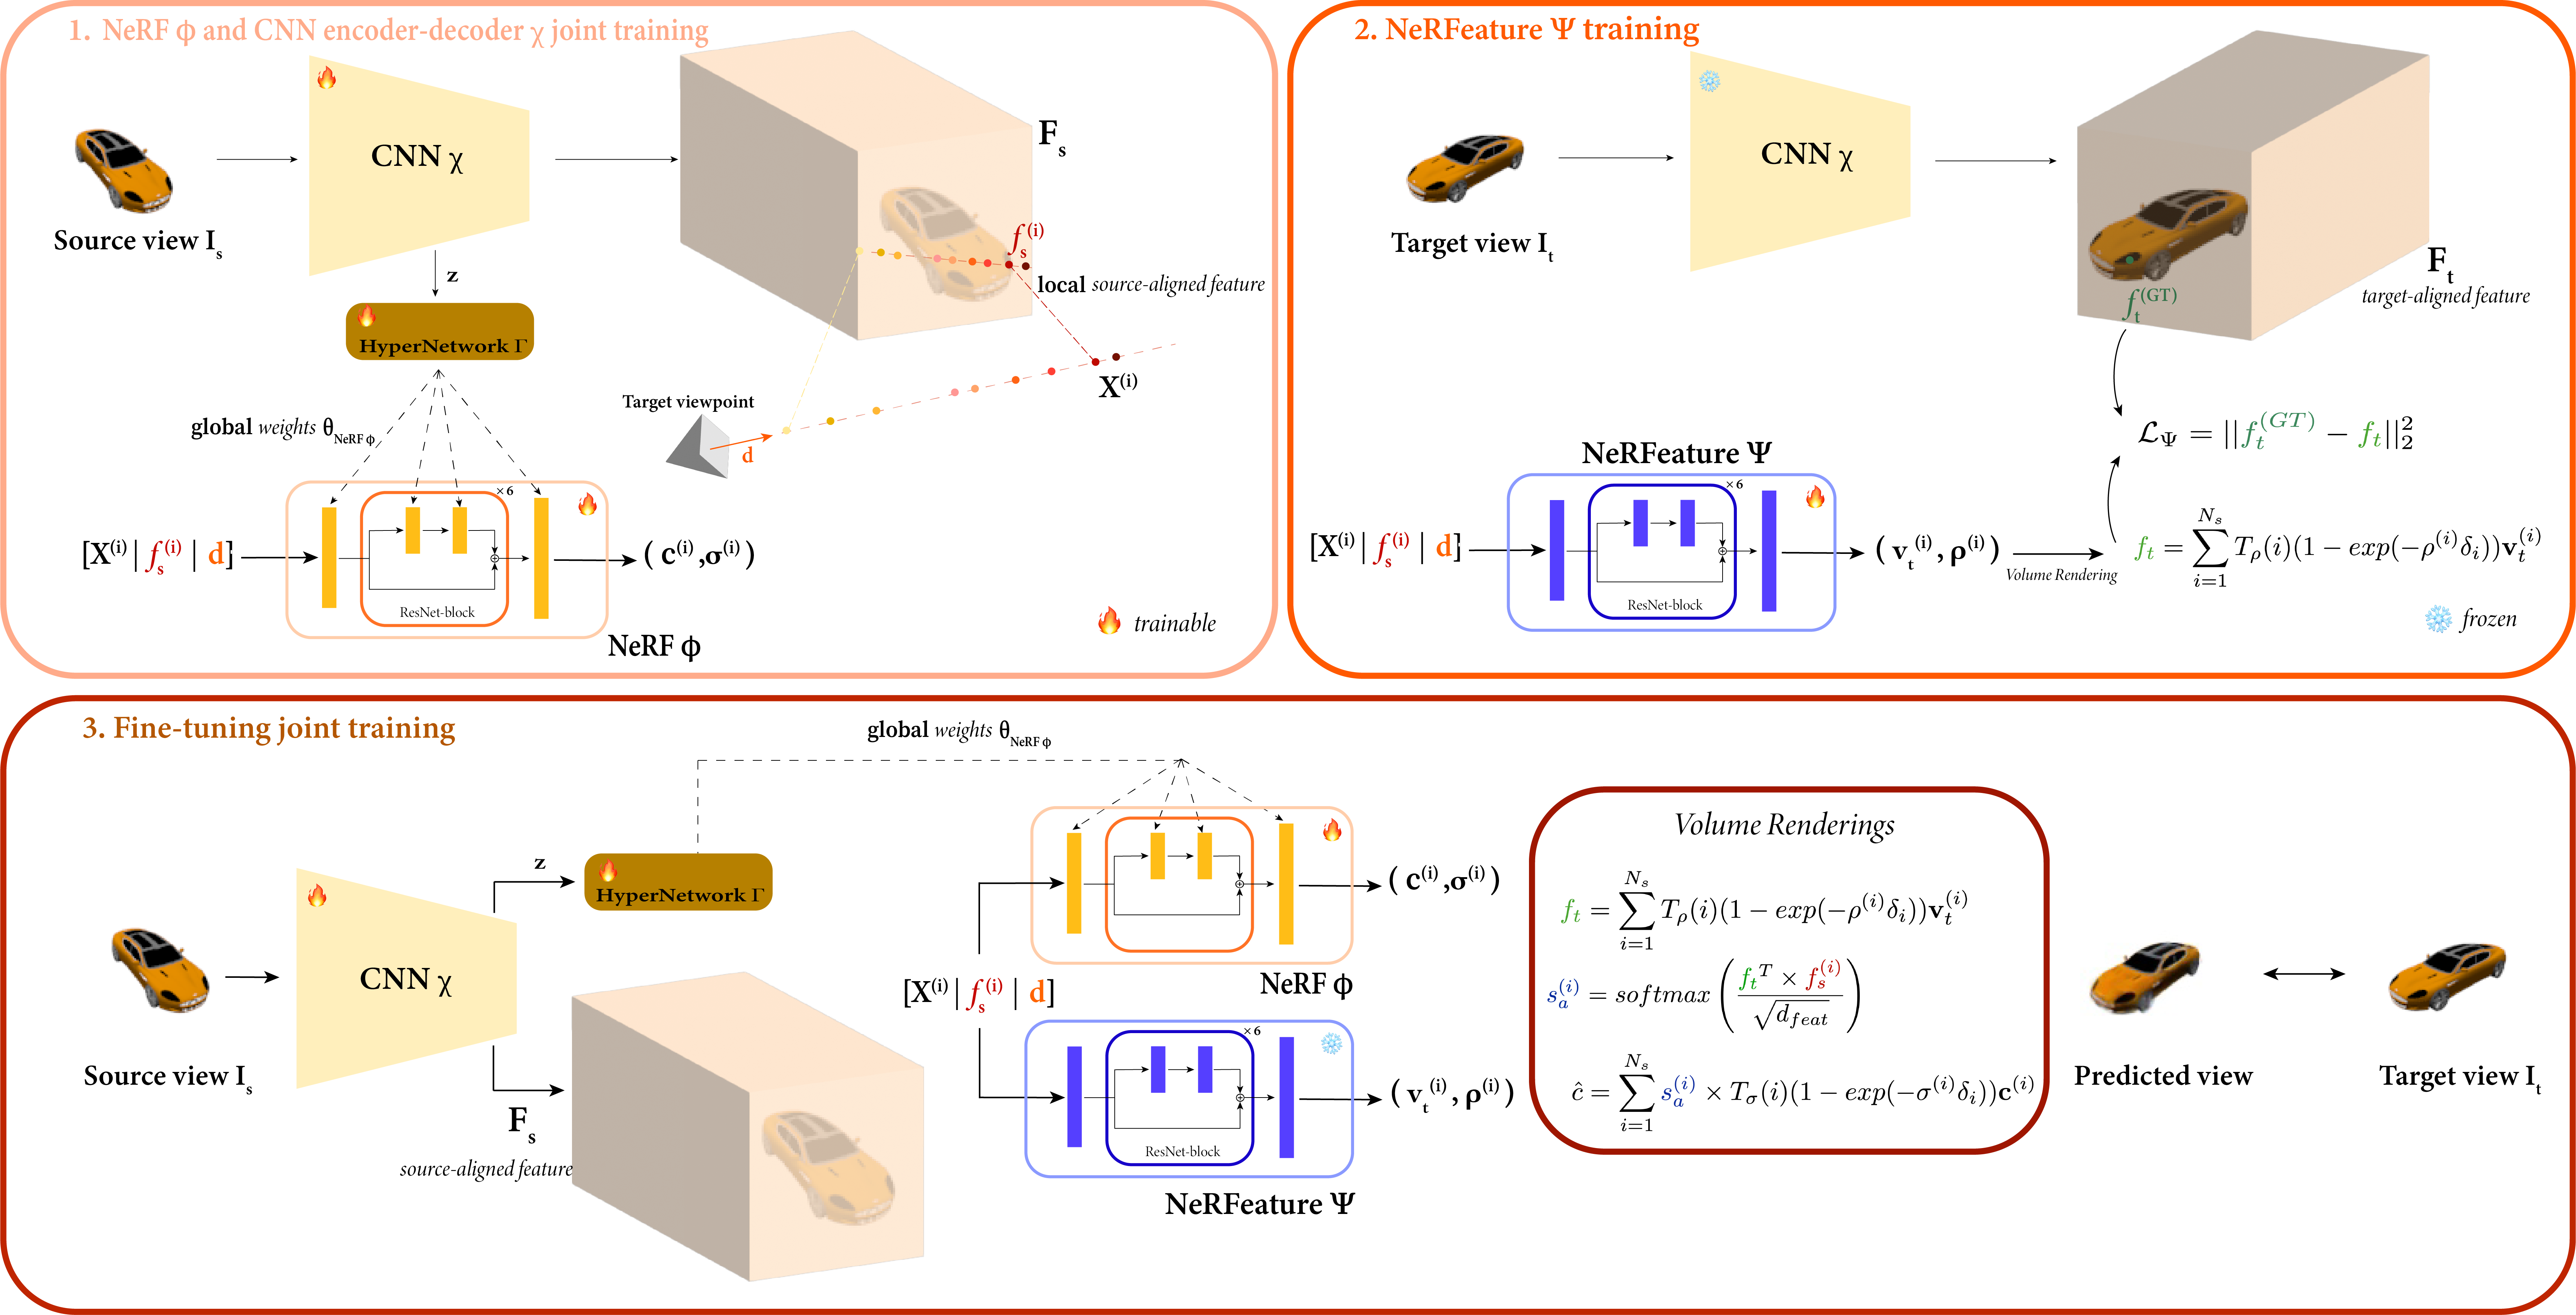
\includegraphics[height=8cm]{images/epinerf/overview_architecture.png}
  \caption{\textbf{Overview of our complete two-stage training EpiNeRF architecture.} (Top left) The first step primarily aims to train our CNN encoder-decoder $\chi$, which can subsequently generates \textit{local} deep features aligned with $I_{s}$. (Top right) Our CNN $\chi$ is then used a teacher model to instruct a residual NeRF student model $\Psi$, termed NeRFeature, to generate such features from any target viewpoint. (Bottom) The second stage training of EpiNeRF is more likely a fine-tuning of both $\chi$ and $\Phi$, with a modified attention epipolar-based volume rendering equation, thanks to the target-aligned feature produced by NeRFeature $\Psi$.}
  \label{fig:overview}
\end{figure*}
\subsection{NeRFeature: learn target-aligned features}
\label{subsec:nerfeature}

While feature volumes produced by any 2D models (CNN or ViT) are defacto aligned with the RGB image they have been fed with (i.e the source image $I_s$), we propose to distil and learn such feature space into 3D through a neural feature radiance field, termed NeRFeature $\Psi$. 

A pretrained teacher 2D CNN encoder $\chi$ (top-left panel on Figure \ref{fig:overview} and subsection \ref{subsec:epinerf}) produces \textit{pseudo} ground truth features, that are used to supervise the training distillation of the NeRFeature $\Psi$ (top-right panel on Figure \ref{fig:overview}).

Given a 3D point $\mathbf{x}^{(i)}$ expressed in the world coordinate system along a ray $\mathbf{r}$ from a target direction $\mathbf{d}$, we denote: 

\begin{equation}
    f_{s}^{(i)} = \mathbf{F}_{s}(\pi(\mathbf{x}^{(i)}))  \in \mathbb{R}^{d_{\text{feat}}} 
    \label{eq:projection}
\end{equation}

the source-aligned feature that was extracted from $\mathbf{F}_{s}=\chi(I_{s})$through the perspective projection $\pi$ of $\mathbf{x}^{(i)}$ on the feature plane.

As the feature radiance field learned through $\Psi$ must be generalizable (\textit{i.e} render meaningful features for unseen objects or scene), NeRFeature has to be input-conditioned on $f_{s}^{(i)}$: 

\begin{equation}
    \Psi(\mathbf{x}^{(i)},\mathbf{d},f_{s}^{(i)}) = (\rho^{(i)},\mathbf{v}_{t}^{(i)}) \in \mathbb{R}_{+}\times \mathbb{R}^{d_{\text{feat}}}
\end{equation}

while the target-aligned feature $\mathbf{f}_{t}$ is obtained through the vanilla volume rendering equation computed over the $N_s$ sampled points on \textbf{r}: 

\begin{equation}
    f_{t} = \sum_{i=1}^{N_{s}} T_{\rho}(i)(1-exp(-\rho^{(i)}\delta_{i}))\mathbf{v}_{t}^{(i)}
\end{equation}

with $\delta_{i}=\mathbf{x}^{(i+1)}-\mathbf{x}^{(i)}$  the distance between two consecutive samples and $T_{\rho}(i) = \exp\left(-\sum_{j=1}^{i}\rho^{(j)}\delta_{j}\right)$ the accumulated transmittance along \textbf{r}.

 Such a learned feature field is finally queried (see Section \ref{subsec:epipolar_att}) during the joint fine-tuning (Figure \ref{fig:overview} - bottom) phase to render target-aligned features, that are involved in an epipolar-based attention mechanism. 
 
\subsection{Feature-based epipolar attention}
\label{subsec:epipolar_att}

As soon as deep feature from $\chi$ has been distilled into the NeRFeature $\Psi$, target-aligned features can be synthesized by solely requiring the source-aligned feature and the corresponding camera relative transformation. A cross-attention distribution \citep{vaswani2017attention} can therefore be computed with such source-aligned features, that all lie on the epipolar line defined by the sampled pixel on the target view. In this way, for any 3D point $\mathbf{x}^{(i)}$, a cross-attention score is obtained from: 

\begin{equation}
    s_{a}^{(i)} = softmax\left(\frac{f_{t}^{T}\times f_{s}^{(i)}}{\sqrt{d_{\text{feat}}}}\right) \in [0,1].
\label{eq:attention}
\end{equation}

The entire distribution $\textbf{s}_{a} \in \mathbb{R}^{N_{s}}$ is obtained by gathering the cross-attention scores for all the $N_s$ projected samples (that all lie on the epipolar line in the source view domain). 

Such an attention score gives an idea of how closed source-aligned features are from the target feature, predicted by $\Psi$. Since it exists an epipolar-based relationship between the location $f_{s}^{(i)}$ and $f_{t}$, the score distribution $\mathbf{s}_{a}$ should has a maximum at the location where target and source pixels exhibit the same content. Associated observation is illustrated on Figure \ref{fig:attention-illustration}. The cross-attention $\mathbf{s}_{a}$ is not used to weight the $\mathbf{f}_{s}$ distribution in the RGB-volume rendering \citep{max1995optical} but rather to adjust the weights distribution $\omega$ that is going to be involved through the inverse transform sampling strategy \citep{mildenhall2020nerf} in the fine NeRF network: 

\begin{equation}
    \omega_{i} = s_{a}^{(i)} \left(1 - \exp(-\delta_{i}\sigma^{(i)})\right)T_{\sigma}(i).
\end{equation}


\subsection{EpiNeRF: the complete architecture}
\label{subsec:epinerf}
\noindent\textbf{CNN-based source-aligned features.} Plethora of recent NeRF-based NVS works leverage their radiance field on a source-aligned feature volume $\mathbf{F}_{s}$, obtained from either a CNN \citep{jang2021codenerf,yu2021pixelnerf,li2022symmnerf} or a ViT \citep{lin2023vision}. However, intermediate features produced by the inner encoder, termed $(\mathbf{F}_{1},\mathbf{F}_{2},\mathbf{F}_{3},\mathbf{F}_{4})$ here,  are often fused and upscaled in a vanilla way, through bilinear upsampling and concatenation in the CNN decoder. The final low-resolution feature volume $\mathbf{F}_{s}$ is obtained through: 
\begin{equation}
    \mathbf{F}_{s} = \left[\mathbf{F}_{1}^{up} || \mathbf{F}_{2}^{up} || \mathbf{F}_{3}^{up} || \mathbf{F}_{4}^{up}\right] \in \mathbb{R}^{2d_{\text{feat}} \times \frac{H}{2} \times \frac{W}{2}}
\end{equation}
where the $[.||.]$ denotes the vanilla concatenation. 

Such a source-aligned feature volume can be built differently, by accounting on residual connections and atrous convolutions, as \citep{chan2023genvs} did too. 
EpiNeRF thus rather gets consideration for DeepLabV3+ \citep{chen2018encoder} as a backbone decoder for the feature volume $\textbf{F}_{s}\in \mathbb{R}^{d_{\text{feat}} \times H \times W}$.  Both upscaling and merging strategies are presented on the Figure \ref{fig:feature_encoder}. 

\begin{figure*}[htb!]
    \center
  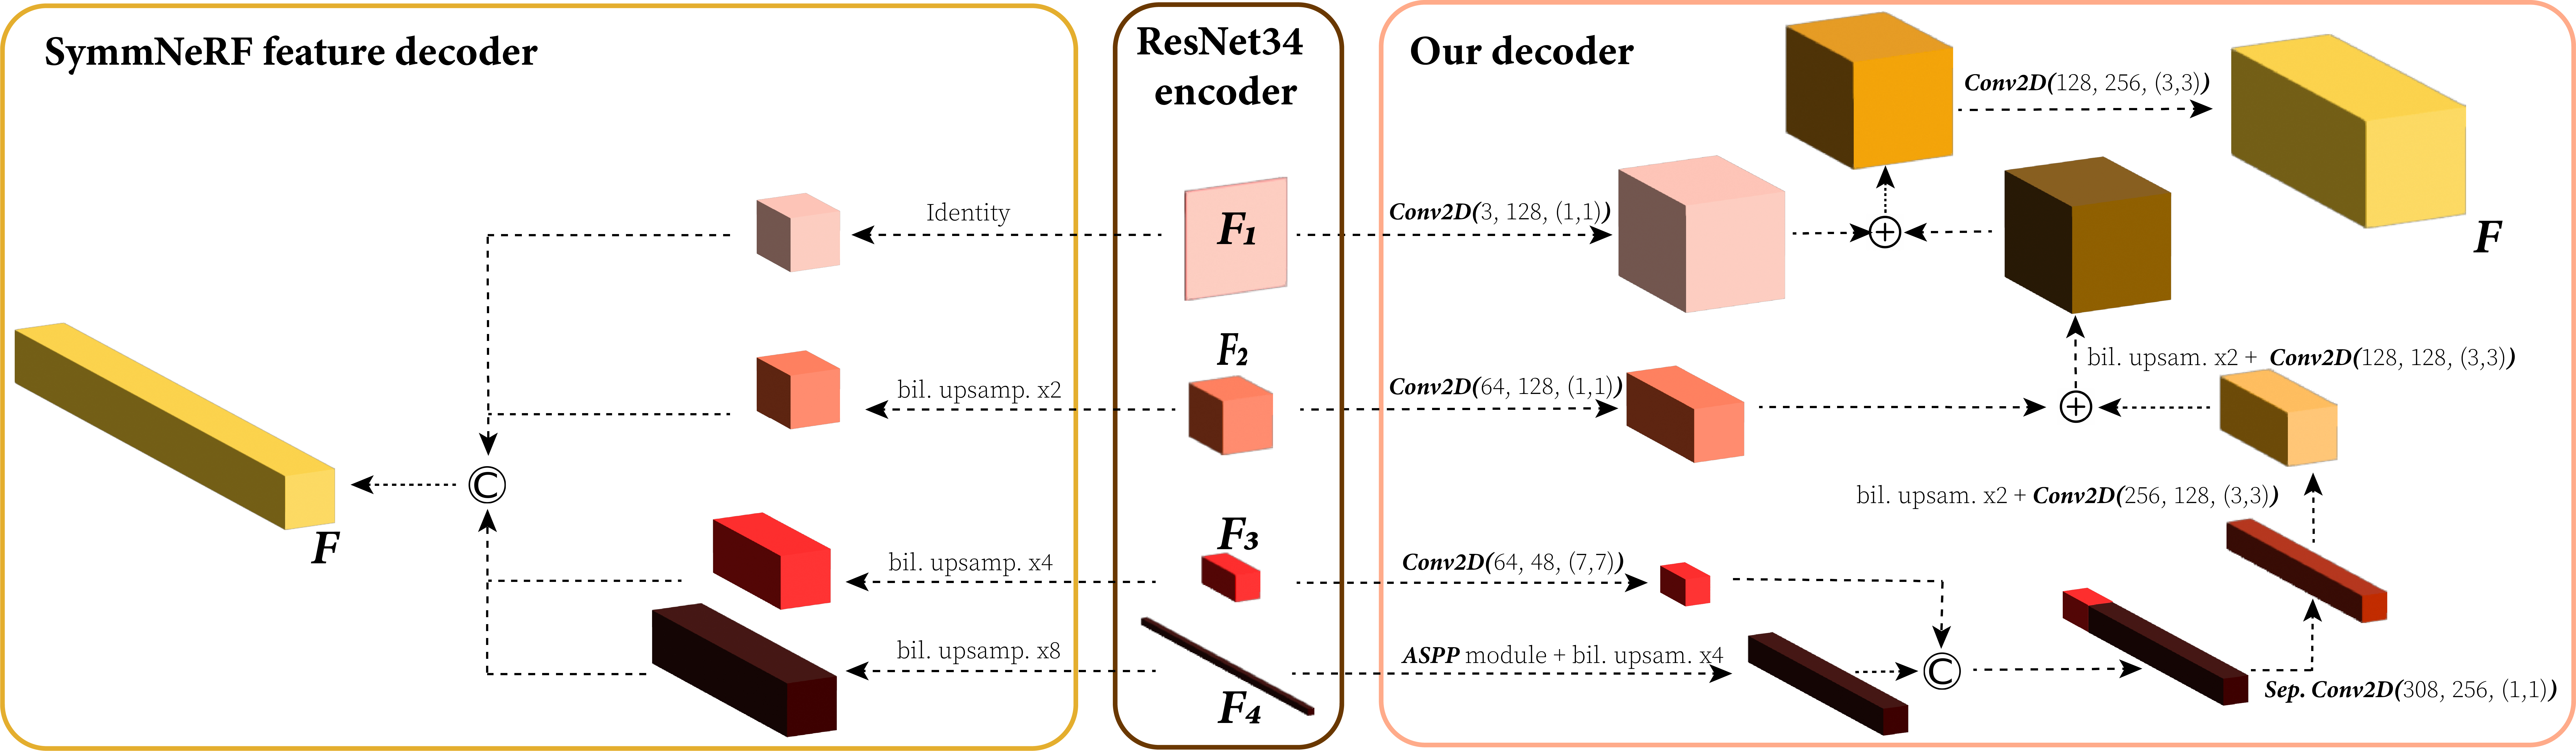
\includegraphics[height=3.5cm]{images/epinerf/feature_fusion_encoder.png}
  \caption{Overview of the CNN decoder $\chi$ involved in SymmNeRF (left) and in our configuration by leveraging on DeepLabV3+ (right). One might note that $\chi$ in both case leverages a ResNet34-based encoder \citep{he2016deep}. }
  \label{fig:feature_encoder}
\end{figure*}
EpiNeRF's feature volume has therefore the same resolution as the input image $\mathbf{I}_s$. While pixel-aligned features are bilinearly interpolated through a 2$\times$2 window, a larger resolution allows better local features sampling that are going to condition the radiance field. \newline

\noindent\textbf{Local and global NeRF conditioning.} Our CNN encoder-decoder $\chi$ primarily produces a set of features $(\mathbf{F}_{1},\mathbf{F}_{2},\mathbf{F}_{3},\mathbf{F}_{4})$ from $\textbf{I}_{s}$. While $\mathbf{F}_{s}$ must be considering as a \textit{local} input conditioning of the radiance fields (since feature are pixel-wise sampled during the perspective projection), we leveraged on an additional MLP network, called a hypernetwork $\Gamma$, that aims to predict NeRF $\Phi$ weights, termed $\theta$, given a latent code $\mathbf{z}$, that is obtained from a non-linear projection of $\mathbf{F}_{4}$. The complete output of our CNN encoder-decoder $\chi$ can thus be re-written as:

\begin{equation}
    \textbf{z}, \textbf{F}_{s} = \chi(I_{s})
\end{equation}
and $\Phi$ is thus  both \textit{locally} (on its input) and  \textit{globally} (through its weights) conditioned: 
\begin{equation}
     \Phi_{\theta}(\mathbf{x}^{(i)},\mathbf{d},f_{s}^{(i)},f_{t}) = (\sigma^{(i)},\mathbf{c}^{(i)}) \hspace{.5cm}\text{;}\hspace{.5cm}  \theta = \Gamma(\mathbf{z})
\end{equation}\newline

\noindent\textbf{Symmetry prior integration.}
Following SymmNeRF \citep{li2022symmnerf} prior work, we made the assumption the (YZ) plane in the canonical coordinates system was a symmetry plane for the implicit 3D scenes we are aiming to reconstruct. It thus involves that a 3D point $\mathbf{x}$ along a target ray \textbf{r} has a symmetrical point with respect to the (YZ)-symmetry plane through:
\begin{equation}
    \mathbf{x}^{(i)}_{symm} = \mathbf{M}\mathbf{x}^{(i)}
\end{equation}
where $\mathbf{M} = \mathbf{I}_{4}\footnote{the Identity matrix in $\mathbb{R}^{4}$} - 2e_{1}e_{1}^{T}$ and $e_{1}$ the first 3D unit basis vector. Such a symmetrical 3D point is back-projected on the source-aligned feature volume $\mathbf{F}_{s}$, as $\mathbf{x}$ was through Equation \eqref{eq:projection}. The \textit{local} deep feature fed to the NeRF $\Phi$ is finally: 
\begin{equation}
    f^{(i)} = \left[f_{s}^{(i)}||f_{s,symm}^{(i)}\right]
\end{equation}

\noindent\textbf{Training.} As depicted on Figure \ref{fig:overview}, our EpiNeRF architecture has a two-step training procedure. It integrates a feature radiance field, termed NeRFeature $\Psi$, in combination with a CNN-based encoder-decoder $\chi$ that \textit{locally} condition the main RGB radiance fields $\Phi$ through an epipolar based attention mechanism. A hypernetwork $\Gamma$ also \textit{globally} conditions $\Phi$, by predicting its learnable parameters through a lightweight MLP network. 

Considering a training set of N objects $\{\mathcal{D}\}_{i=1}^{N}$ with V different viewpoints $\mathcal{D}^{(i)} = \{I_{i}^{(j)},\pi_{i}^{(j)}\}_{j=1}^{V}$ per instance and a batch of rays $\mathcal{R}$, EpiNeRF is optimised through the loss functions: 
\begin{equation}
 \min_{\Psi} \sum_{i}\sum_{j}\mathcal{L}_{\Psi}\left(I_{i}^{(j)},\pi_{i}^{(j)},\Psi,\chi \right) \hspace{.2cm} ; \hspace{.2cm}\mathcal{L}_{\Psi}= \sum_{\mathbf{r}\in\mathcal{R}} || f_{t}(\mathbf{r}) - f_{t}^{(GT)}(\mathbf{r}) ||_{2}^{2}
\end{equation}
and 
\begin{equation}
 \min_{\zeta=\{\chi,\Phi,\Gamma\}}\sum_{i}\sum_{j}\mathcal{L}_{\zeta}\left(I_{i}^{(j)},\pi_{i}^{(j)},\Psi,\zeta \right)\hspace{.2cm}  ; \hspace{.2cm}\mathcal{L}_{\zeta}= \sum_{\mathbf{r}\in\mathcal{R}} || c(\mathbf{r}) - c^{(GT)}(\mathbf{r}) ||_{2}^{2}
\end{equation}


where $c^{(GT)}(\mathbf{r})$ represents the ground truth pixel that was sampled on $\mathbf{I}_{t}$, $f^{(GT)}(\mathbf{r})$ the \textit{pseudo} ground truth deep feature that was sampled $F_{t}=\chi(I_{t})$.
\newline

Deep features produced by NeRFeature are implicitly input-conditioned by $\chi$ since the source aligned feature $f_s^{(i)}$ is fed as input. Hypernetwork $\Gamma$ finally does not have to be trained with a specific loss objective: weights are updated during back-propagation through the vanilla $\mathcal{L}_{2}$ loss function defined over the sampled RGB pixels. 

The second fine tuning training stage is trained in a similar way to the first one, even though NeRFeature weights are now frozen to produce target-aligned features. 

We followed the training strategy that SymmNeRF \citep{li2022symmnerf} and VisionNeRF \citep{lin2023vision} used for $\chi$ and $\Phi$ in both stages and formed batches of 4 images during training, averaged our loss function over 256 rays, and sampled a total of $N_{s}=192$ points along each ray.

\section{Experiments}
\subsection{View synthesis on synthetic data - SRN ShapeNet}
The first presented results were obtained on the ShapeNet dataset \citep{chang2015shapenet}, by focusing on the ShapeNet-SRN \citep{sitzmann2019scene} version. The \textit{Cars} and \textit{Chairs} classes respectively have 3514 and 6591 objects. Training is performed over the 50 different views per instance, while the testing set has 251 views per object, sampled on an Archimedean spiral. We adopted the same evaluation strategy all related works used and considered the view $64^{th}$ as the source image $\textbf{I}_{s}$. Results have been  averaged over the remaining 250 target views. 

Our method reaches state-of-the-art performances according to Table \ref{table:comp_res} and even outperforms the heavier transformer-based architecture \citep{lin2023vision} on almost all metrics. 

\begin{table}[htp!]
\caption{Comparisons against state of the art methods on the category specific \textit{Chairs} and \textit{Cars} classes from the ShapeNet-SRN dataset. Best results are highlighted in red, second ones in orange and third ones in yellow. }
\label{table:comp_res}
\centering%\begin{center}
\begin{adjustbox}{height=2.3cm}
\begin{tabular}[h]{c||ccccccc}
\hline
 Method & \multicolumn{3}{c}{Car} & \multicolumn{3}{c}{Chair} \\
 &  SSIM ($\uparrow$) & PSNR ($\uparrow$) & LPIPS ($\downarrow$) & SSIM ($\uparrow$) & PSNR ($\uparrow$)) & LPIPS ($\downarrow$)\\
\hline
SRN \citep{sitzmann2019scene}& \cellcolor{yellow!25}0.89 & 22.25 & 0.129 & 0.89 & 22.89 & 0.104\\
PixelNeRF \citep{yu2021pixelnerf} & \cellcolor{orange!25}0.90 & 23.17 & 0.146 & \cellcolor{yellow!25}0.91 & 23.72 & 0.128\\
FE-NVS \citep{guo2022fast} & \cellcolor{red!25}0.91 & 22.83 & \cellcolor{yellow!25}0.099 & \cellcolor{orange!25}0.92 & 23.21 & 0.077 \\
GeNVS\citep{chan2023genvs}& \cellcolor{yellow!25}0.89 & 20.7 & 0.104 & - & - & - \\
ShaRF \citep{rematas2021sharf} & \cellcolor{orange!25}0.90 & 22.90 & - & \cellcolor{orange!25}0.92 & 23.37 & - \\
CodeNeRF \citep{jang2021codenerf} & \cellcolor{red!25}0.91 & \cellcolor{orange!25}23.80 & - & 0.90 & 23.66 & -  \\
SymmNeRF\footnotemark\citep{li2022symmnerf}& \cellcolor{orange!25}0.90 & \cellcolor{yellow!25}23.10 & 0.110 & \cellcolor{yellow!25}0.91 & \cellcolor{yellow!25}24.14  & \cellcolor{orange!25}0.075 \\
VisionNeRF \citep{lin2023vision} & \cellcolor{red!25}0.91 & 22.88 & \cellcolor{orange!25}0.084 & \cellcolor{red!25}0.93 & \cellcolor{red!25}24.48  & \cellcolor{yellow!25}0.077 \\
Ours &\cellcolor{red!25} 0.91 & \cellcolor{red!25}24.01 &\cellcolor{red!25} 0.082 &  \cellcolor{orange!25} 0.92 & \cellcolor{orange!25}24.30 & \cellcolor{red!25}0.072 \\

\hline 
\end{tabular}
\end{adjustbox}
%\end{center}
\end{table}
\footnotetext[3]{SymmNeRF\citep{li2022symmnerf} results differ from the ones originally reported by authors since we had to retrain their architecture.}

As depicted in Figure \ref{fig:exp-srn-car}, EpiNeRF successfully gathers best aspects of both SymmNeRF \citep{li2022symmnerf} and VisionNeRF \citep{lin2023vision}. It renders novel views that are simultaneously sharp (eased by the ViT in VisionNeRF) and consistent from a symmetrical perspective on colour patterns (eased by the symmetry prior from SymmNeRF). In this regard, the red left rear door, that is not observed in the source view of the first row,  the right front light on the second one or the white trim in the last example are accurately synthesized by our architecture, contrary to concurrent works that either fail to synthesise sharp views (SymmNeRF) or grasp inherent symmetrical patterns (VisionNeRF). Having a higher-resolution feature volume \textbf{F} helps the radiance field generate sharper results, as shown in section \ref{subsec:visual_insights}. 

\begin{figure}[htb!]
    \center
  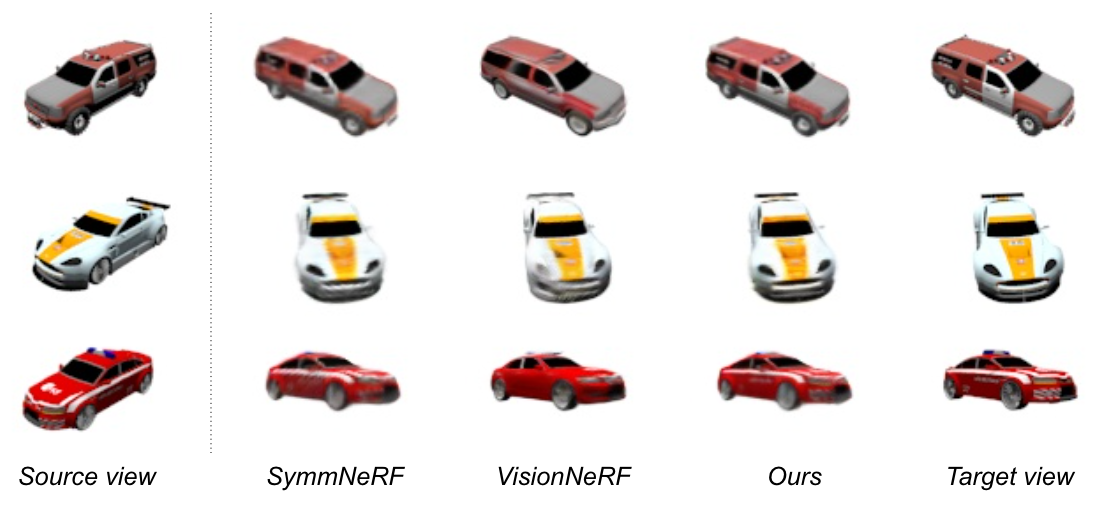
\includegraphics[height=5cm]{images/epinerf/exp-srn-cars.png}
  \caption{Novel view synthesis on the category-specific \textit{Cars} class from ShapeNet. Our method allows to render sharper novel views than SymmNeRF \citep{li2022symmnerf} while maintaining the symmetry that VisionNeRF \citep{lin2023vision} fails to preserve.}
  \label{fig:exp-srn-car}
\end{figure}

 Similar observations can be drawn from the \textit{Chairs} class in Figure \ref{fig:exp-srn-chair}. Intricate geometry on the back and armrests is not entirely synthesised by VisionNeRF  which fails to apprehend how symmetric a chair can be: the armrest structure on the first row is partially missing in the rendered view, even though all the visual information was provided in the source view to render it. SymmNeRF suffers from the same blurry rendering issue that was pointed out in the \textit{Cars} class. Our method offers the best compromise regarding detail retrieval and symmetry reasoning compared to state-of-the-art methods.
 
\begin{figure}[htb!]
    \center
  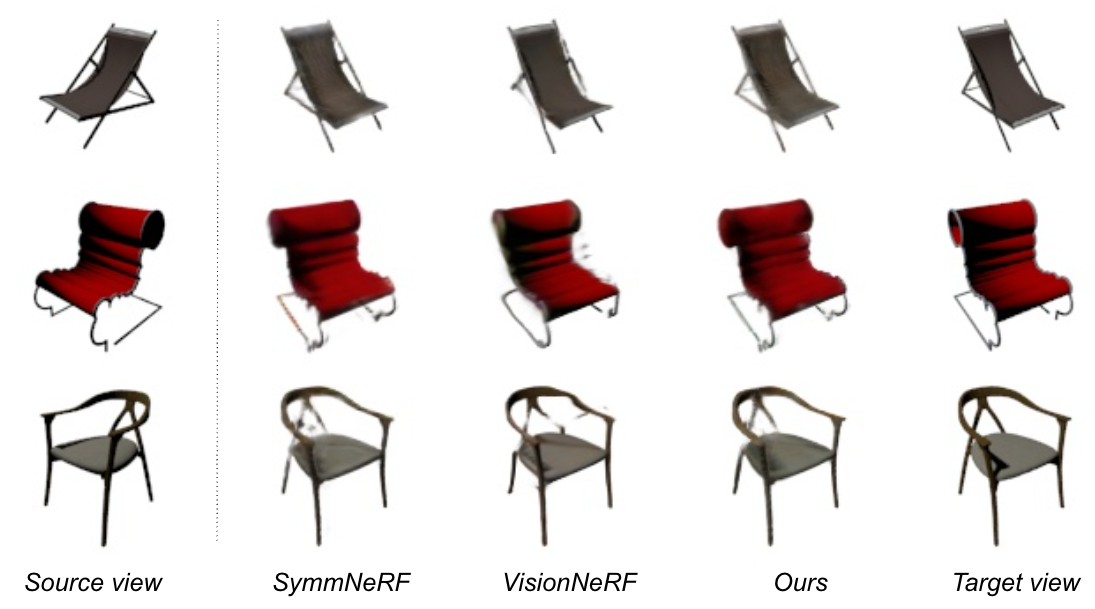
\includegraphics[height=6.1cm]{images/epinerf/exp-srn-chairs.png}
  \caption{Novel view synthesis on the category-specific \textit{Chairs} class from ShapeNet. Tiny structures are not entirely rendered by \citep{li2022symmnerf,lin2023vision} whereas our method manages to reproduce complex back or armrest structures.}
  \label{fig:exp-srn-chair}
\end{figure}

\subsection{View synthesis on real data}
We evaluate our EpiNeRF architecture on real world images, by focusing on the Stanford Cars dataset \citep{krause20133d}. While raw images have been segmented using state-of-the art segmentation model SAM \citep{kirillov2023segment}, images have also been scaled and centred accordingly to match as closed as possible the ShapeNet-SRN image structure. If such a testing scenario is far from the one our architecture has been trained for, Figure \ref{fig:res_Stanfordcar} shows how EpiNeRF is able to produce sharper results than SymmNeRF \citep{li2022symmnerf}, even without any reliable camera pose information.

\begin{figure}[htb!]
    \center
  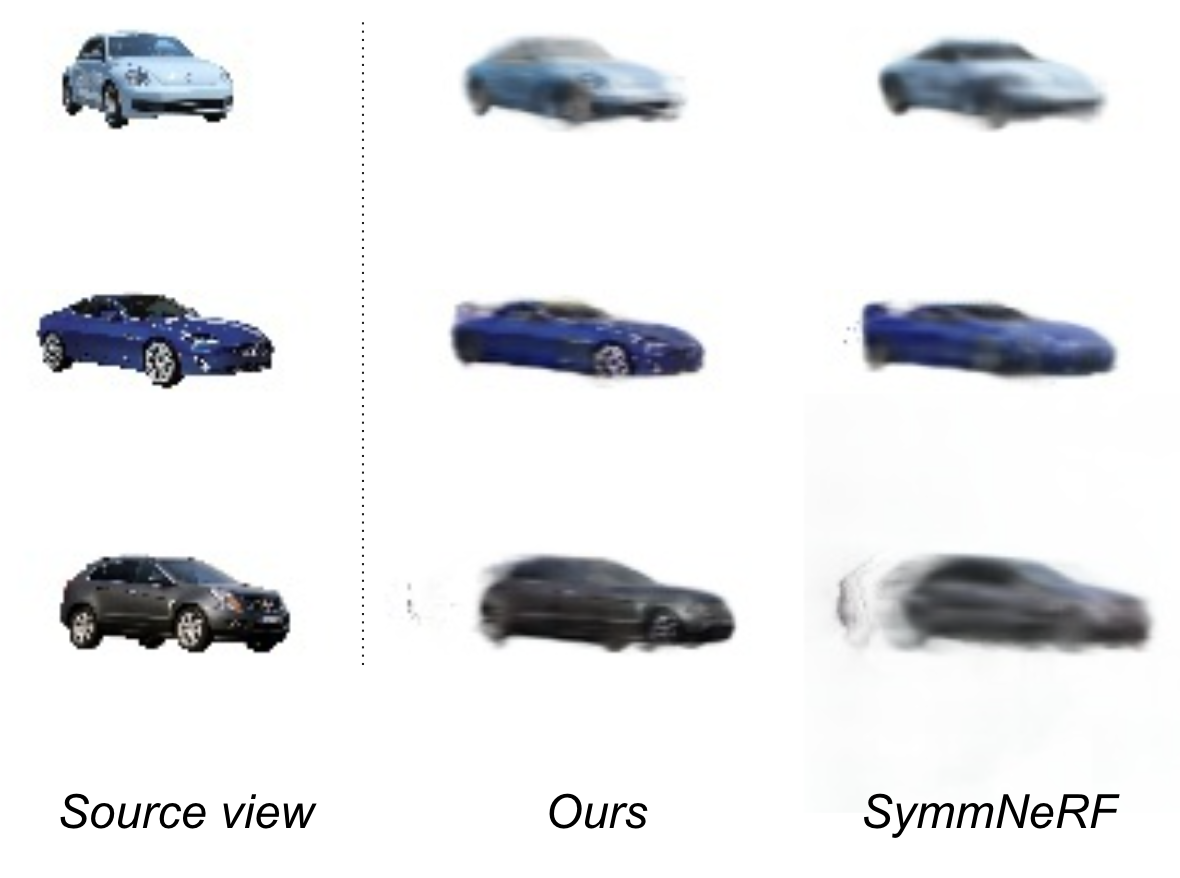
\includegraphics[height=6.cm]{images/epinerf/res_standford_cars.png}
  \caption{Novel view synthesis on the few real \textit{Cars} from the Stanford dataset \citep{krause20133d}. Whereas even closed target viewpoint from the source view leads to fuzzy results, our method render sharper results than SymmNeRF \citep{li2022symmnerf}. }
  \label{fig:res_Stanfordcar}
\end{figure}



\subsection{Ablation study}
Starting with a \textit{baseline} architecture that integrates no symmetry prior information, a vanilla bilinear upsampling strategy to produce $\mathbf{F}_{s}$ and no epipolar attention, we conducted an ablation study to show in which extent each EpiNeRF's components behave on our final novel view rendering architecture. 

\begin{table}[htp!]
\caption{Influence of the different modules onto the final EpiNeRF architecture.}
\label{tab:ablation}
%\begin{center}
\centering
\begin{adjustbox}{width=\textwidth}
\begin{tabular}[h]{c||ccccccc}
\hline
Method & \multicolumn{3}{c}{Car} & \multicolumn{3}{c}{Chair} \\
 &  SSIM ($\uparrow$) & PSNR ($\uparrow$) & LPIPS ($\downarrow$) & SSIM ($\uparrow$) & PSNR ($\uparrow$)) & LPIPS ($\downarrow$)\\[.5pt]
\hline
baseline & 0.89 & 22.71 & 0.108 & 0.90 & 23.03 & 0.090 \\[1.5pt]
\hline 
+ Symmetry constraint \citep{li2022symmnerf}  & \ 0.90 & 23.10  & 0.110 & 0.91 & 24.14 & 0.075 \\
+ DeepLabV3 CNN encoder  & \cellcolor{red!25}{0.91} & 23.87 & 0.087 & \cellcolor{red!25}{0.92} & 24.23 & 0.073 \\
+ Epipolar Attention  & \cellcolor{red!25}0.91 & \cellcolor{red!25}24.01 &\cellcolor{red!25}0.082 & \cellcolor{red!25}0.92 &  \cellcolor{red!25}24.30 &\cellcolor{red!25}0.072 \\
\end{tabular}
\end{adjustbox}
%\end{center}

\end{table}

As shown on Table \ref{tab:ablation} and visually confirmed on Figure \ref{fig:ablation}, integrating the symmetry prior helps the network to better grasp symmetrical and complex pattern structures, whereas the high-resolution feature volume produced by our encoder-decoder $\chi$ leads to sharper edges and thinner structures in RGB space. Finally, the feature attention-based epipolar module, that involved both source-aligned (from $\chi$) and target-aligned (from NeRFeature $\Psi$) features improves the overall quality of the EpiNeRF rendering. 

\begin{figure}[htp!]
    \center
  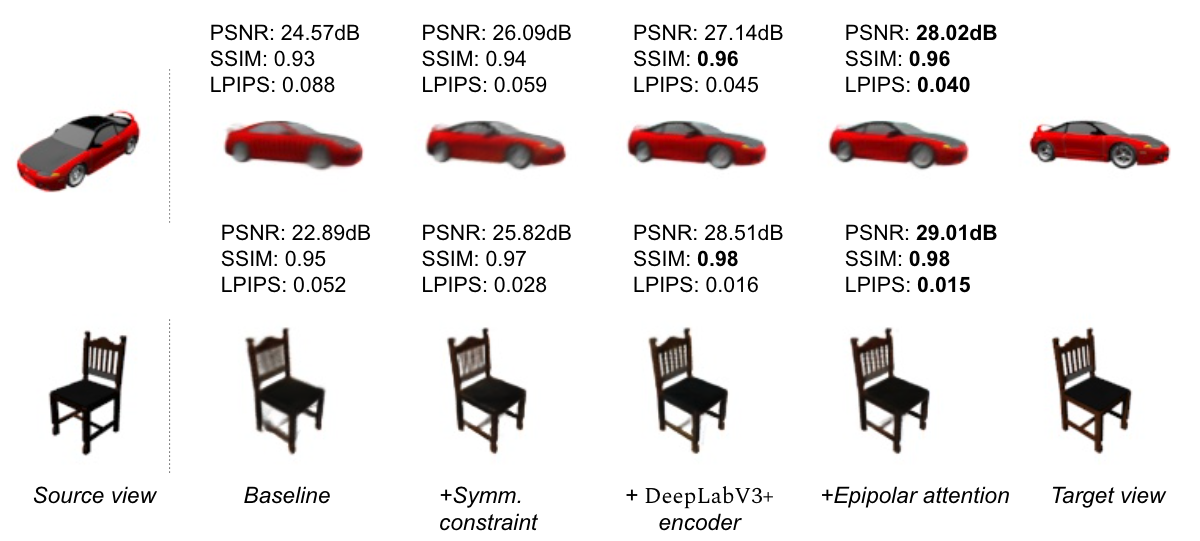
\includegraphics[height=5cm]{images/epinerf/ablation-srn.png}
  \caption{Visual influence of the different modules and constraints that were progressively applied to our architecture on ShapeNet-SRN dataset.}
  \label{fig:ablation}
\end{figure}


\subsection{Feature and attention visual insights}
\label{subsec:visual_insights}


\paragraph{Target-aligned feature synthesis with NeRFeature.} 
Whereas primary purpose of NeRFeature is not to generate an entire feature map from a target viewpoint, one can generate such an $\mathbf{F}_{t}$ deep volume given a source image $I_{s}$ and a corresponding relative camera transformation. Results are depicted on Figure \ref{fig:nerfeature_prediction}. 

\begin{figure*}[htb!]
  \centering
  \begin{subfigure}[t]{0.45\linewidth}
    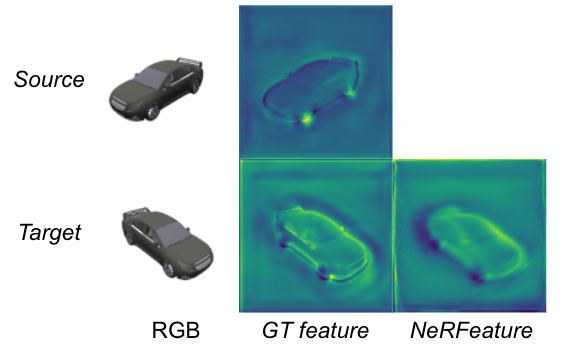
\includegraphics[height=3cm]{images/epinerf/nerfeature.png}
    \caption{\textit{Pseudo} ground truth features are generated through our CNN encoder-decoder $\chi$. Only the first channel are depicted shown for an illustrative purpose.}
    \label{fig:nerfeature_prediction}
  \end{subfigure}
  \hfill
  \begin{subfigure}[t]{0.51\linewidth}
    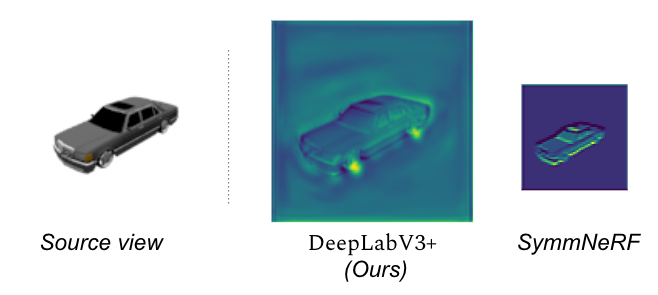
\includegraphics[height=3.cm]{images/epinerf/feature_visuals.png}
    \caption{Feature map \textbf{F} produced by our encoder (\textit{center}, 128$\times$128 spatial res.) and by SymmNeRF (\textit{left}, 64$\times$64 spatial res.) given a source view (\textit{right}, 128$\times$128 spatial res.)}
    \label{fig:featuremap_comparison}
  \end{subfigure}
  \caption{Feature map respectively observed from a target - NeRFeature $\Psi$, \ref{fig:nerfeature_prediction} - and source - CNN $\chi$, \ref{fig:featuremap_comparison} - viewpoint perspective. }
  \label{fig:short}
\end{figure*}

As observed, the overall pose of the target-aligned feature is properly inferred by our feature radiance field $\Psi$, even through tiny details fails to be accurately retrieved (e.g on windows). 

\begin{figure*}[htb!]
  \centering
  \begin{subfigure}[t]{0.48\linewidth}
    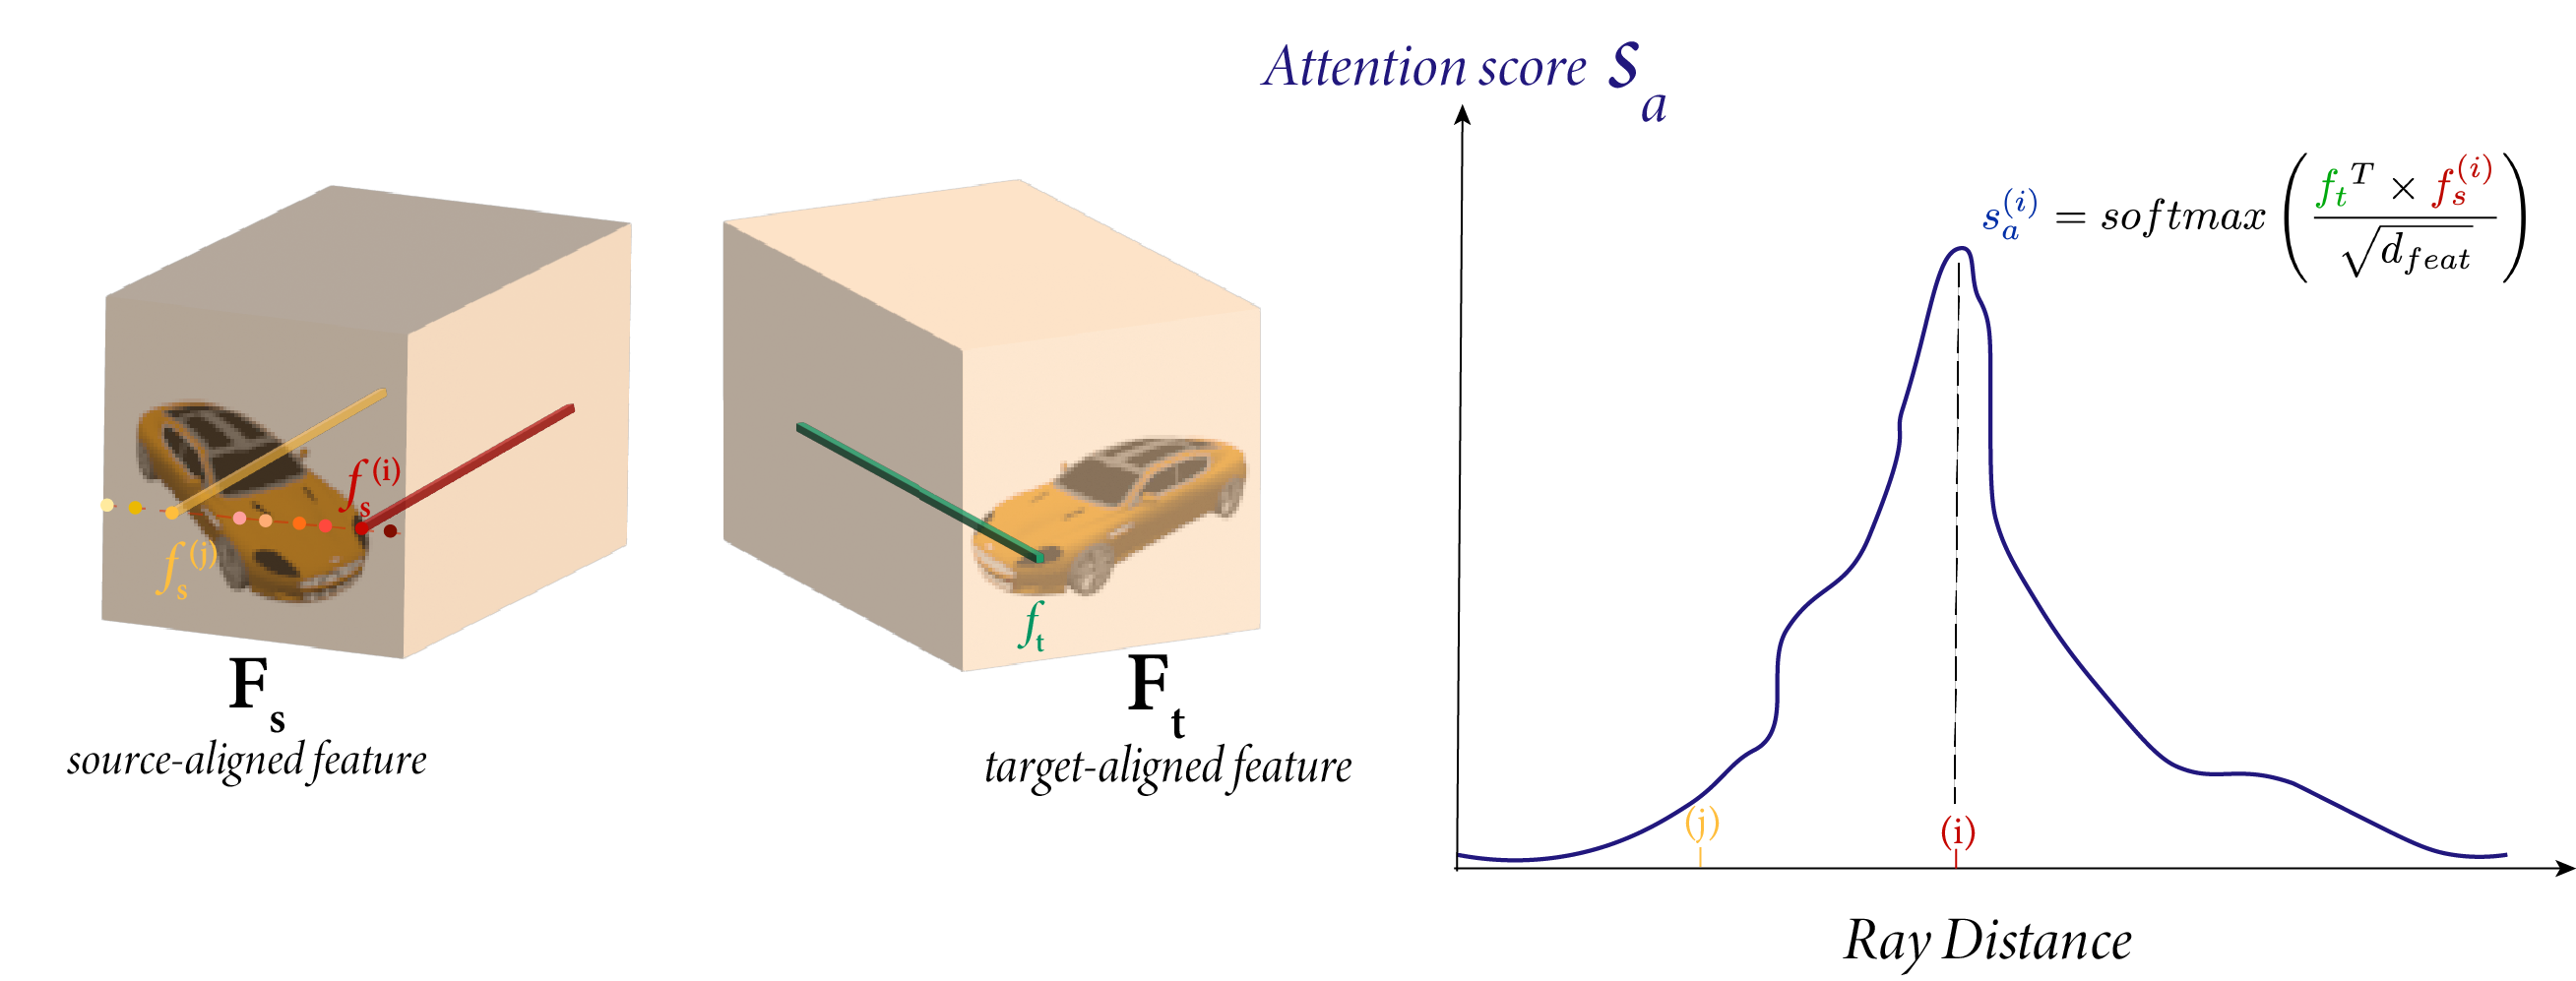
\includegraphics[height=2.4cm]{images/epinerf/attention_illustration.png}
    \caption{Toy feature attention distribution example along a ray. Two closed features that respectively lie in the source and target-aligned feature volume should exhibit a high cross-attention score.}
    \label{fig:attention-illustration}
  \end{subfigure}
  \hfill
  \begin{subfigure}[t]{0.48\linewidth}
    \center
    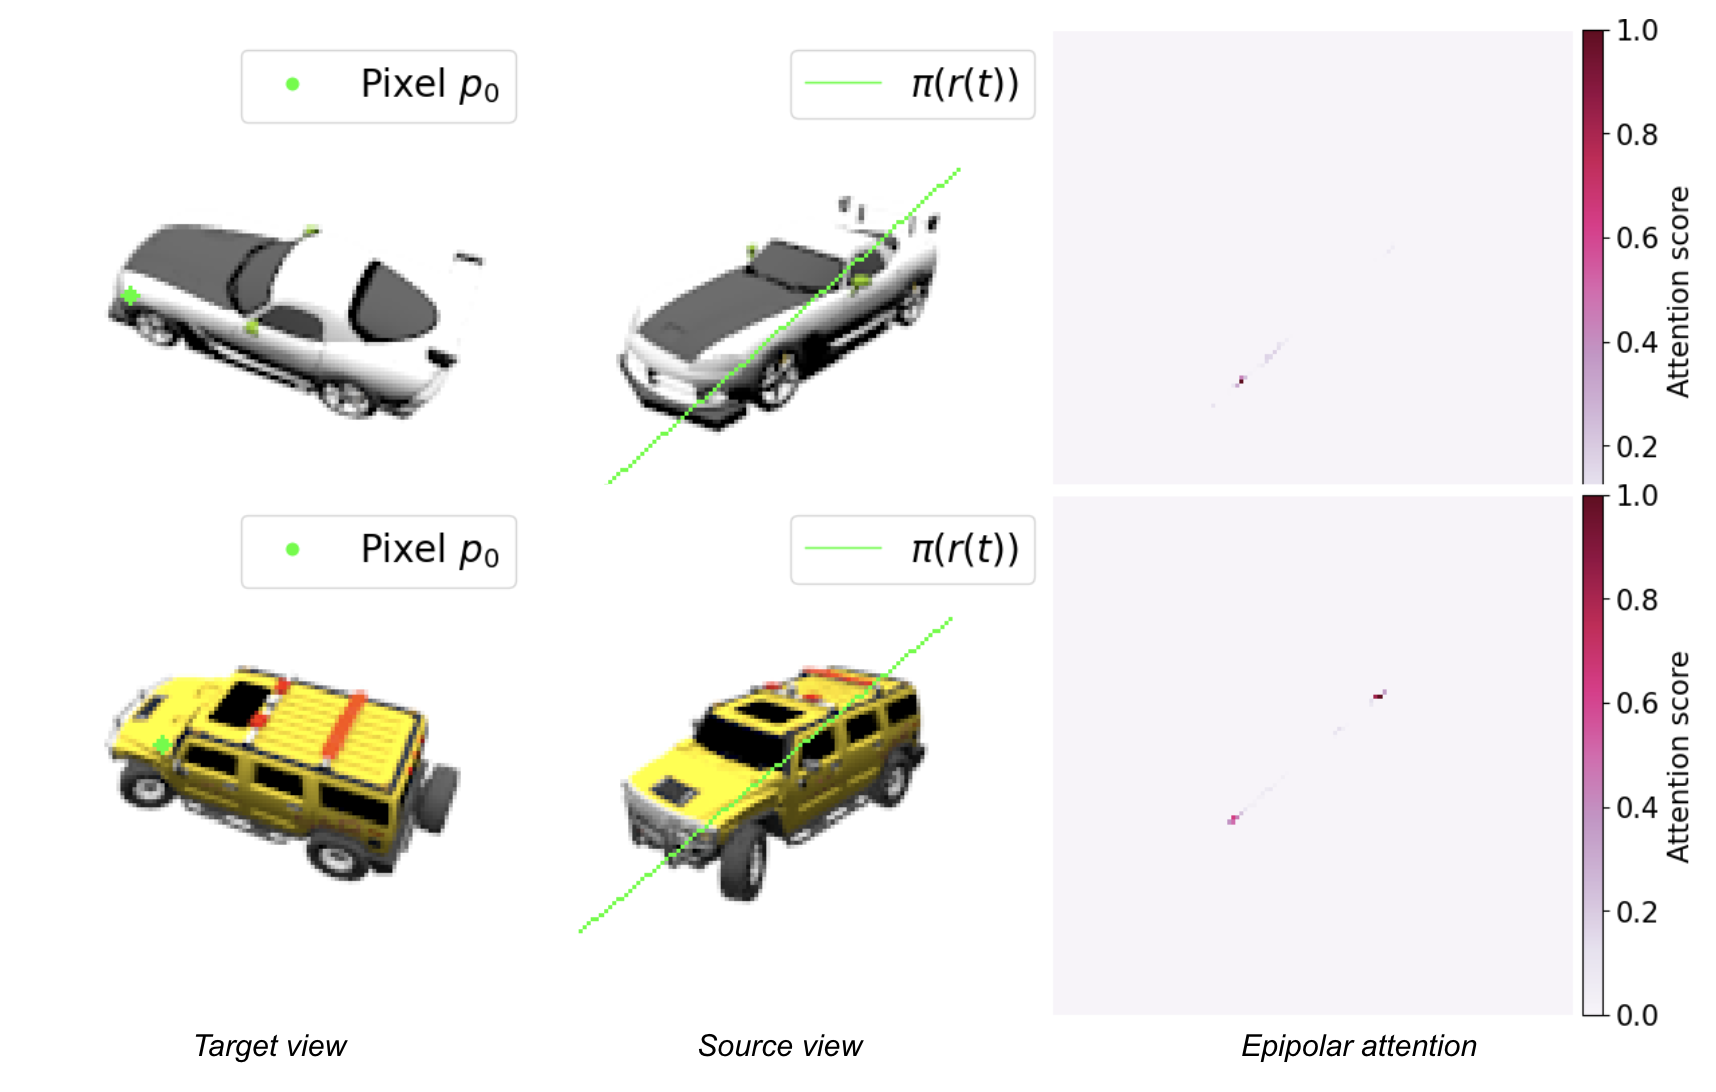
\includegraphics[height=3.3cm]{images/epinerf/exp_epipolar_attention.png}
    \caption{Epipolar attention activation in two different scenarios: While sampling empty area results in low attention scores across the whole epipolar line (top row), proper car areas sampling lead to tightened attention distribution (bottom row).}
    \label{fig:attention-practice}
  \end{subfigure}
  \caption{ \ref{fig:attention-illustration} Source-target feature attention conceptual idea along a ray. \ref{fig:attention-practice} In-practice epipolar-based attention distribution on two instances.}
  \label{fig:attention}
\end{figure*}





\paragraph{CNN encoder-decoder $\chi$.}
Since the EpiNeRF's feature map has the spatial resolution of the source view, first layers of $\textbf{F}_{s}$ should exhibit sharper edges and details compared to SymmNeRF. Figure \ref{fig:featuremap_comparison} tends to confirm such claim: complex regions as on the front part of the car are more coarse in SymmNeRF than on our feature map. Our feature maps are, by design, twice as resolved as those of SymmNeRF, achieving a resolution of $128\times128$. 


\paragraph{Epipolar attention.}
We depict in this last subsection some visuals insights regarding our epipolar attention module. As shown on the second row of Figure \ref{fig:attention-practice}, sampling a target pixel on the yellowish front part of the car will, on the corresponding epipolar line, results in the highest activation closed to the same regions, in the source view domain. 

\section{Limitations \& future work}
While our work address several drawback in existing state-of-the-art methods through the design of target-aligned features, room remains for additional investi\--gations in future works. As the NeRFeature $\Psi$ is an complementary network in our EpiNeRF architecture, inference time is slower than the baseline architecture we considered. However, instead of using two NeRFs ($\Phi$ and $\Psi$) in our EpiNeRF model, one can explore the possibility of only using a single radiance field, namely ($\Phi$), with an additional inner branch devoted to the prediction of the target-aligned features. Such improvement should decrease the inference time closed to the baseline we worked on. 


\section{Conclusion}

In this paper, we propose a new NeRF-based single-image NVS architecture. The NeRF architecture relies on an original CNN-based \textit{local} and \textit{global} conditioning; local since the CNN representation of the source image pixels is used as NeRF's input and global as the whole learnable NeRF's weights are obtained via an hypernetwork that leverages last CNN's layer. The proposed method can thus be summarised as follow: 1) A first NeRF is leaned to give access to high resolution source-aligned features ; 2) This set of features is distilled by the training a second radiance field, termed NeRFeature, that aims to predict high resolution target-aligned features. These two NeRFs and the CNN that conditioned them are merged together to form the proposed EpiNeRF architecture; 3) In a final stage, EpiNeRF is fine-tuned. EpiNeRF main innovation lies on the epipolar constraint that is implemented in the RGB volume rendering via a feature-based attention mechanism. The main strength of such a constraint lies on its $d_{\text{feat}}$-dimensional computation, using a softmax score obtained from both source and target-aligned features. Theses contributions enables EpiNeRF to improved 3D points sampling and consequently achieve a more realistic final rendering result compared to current state-of-the-art methods. We demonstrated our claims on synthetic and real-world datasets, pushing towards better integration of 3D priors including epipolar and symmetrical constraints within generalizable NeRF architectures. 
  






